\documentclass{article}

% if you need to pass options to natbib, use, e.g.:
%     \PassOptionsToPackage{numbers, compress}{natbib}
% before loading neurips_2018

% ready for submission
% \usepackage{neurips_2018}

% to compile a preprint version, e.g., for submission to arXiv, add add the
% [preprint] option:
%     \usepackage[preprint]{neurips_2018}

% to compile a camera-ready version, add the [final] option, e.g.:
     \usepackage[final]{neurips_2018}

% to avoid loading the natbib package, add option nonatbib:
%     \usepackage[nonatbib]{neurips_2018}

\usepackage[utf8]{inputenc} % allow utf-8 input
\usepackage[T1]{fontenc}    % use 8-bit T1 fonts
\usepackage{hyperref}       % hyperlinks
\usepackage{url}            % simple URL typesetting
\usepackage{booktabs}       % professional-quality tables
\usepackage{amsfonts}       % blackboard math symbols
\usepackage{nicefrac}       % compact symbols for 1/2, etc.
\usepackage{microtype}      % microtypography
\usepackage{amsmath}
\usepackage{amssymb}
\usepackage{graphicx}
\usepackage{makecell}
\usepackage{subcaption}
\usepackage{booktabs}

\newcommand{\pd}[2]{\frac{\partial #1}{\partial #2}}
\newcommand{\nl}{\newline}

\title{Deep Learning\\Assignment 2: Recurrent Neural Networks and Graph Neural Networks}

% The \author macro works with any number of authors. There are two commands
% used to separate the names and addresses of multiple authors: \And and \AND.
%
% Using \And between authors leaves it to LaTeX to determine where to break the
% lines. Using \AND forces a line break at that point. So, if LaTeX puts 3 of 4
% authors names on the first line, and the last on the second line, try using
% \AND instead of \And before the third author name.

\author{%
  Daniel Daza\\
  University of Amsterdam\\
  \texttt{daniel.dazacruz@student.uva.nl} \\
}

\begin{document}
% \nipsfinalcopy is no longer used

\maketitle

\begin{abstract}
In this work we are concerned with two architectures widely used in deep learning: Recurrent Neural Networks (RNN) and Graph Neural Networks (GNN). We study the properties of gradients in an RNN and we implement it, as well as the Long Short-Term Memory network (LSTM). We carry out experiments on sequence prediction and text generation, and we analyze the effect of sequence length on these architectures. Lastly, we examine the propagation rule of Graph Convolutional Networks, and explore its properties and applications in comparison to RNNs.
\end{abstract}

\section{Vanilla RNN versus LSTM}

\subsubsection*{Question 1.1}

The equations for the RNN are the following:

\begin{align}
\mathbf{h}^{(t)} &= \tanh(\mathbf{W}_{hx}\mathbf{x}^{(t)} + \mathbf{W}_{hh}\mathbf{h}^{(t-1)} + \mathbf{b}_h) \label{eq:rnn1}\\
\mathbf{p}^{(t)} &= \mathbf{W}_{ph}\mathbf{h}^{(t)} + \mathbf{b}_p\\
\hat{\mathbf{y}} &= \text{softmax}(\mathbf{p}^{(T)}) \\
\mathcal{L} &= -\sum_{k=1}^K y_{k} \log\hat{y}_k \label{eq:rnn2}
\end{align}

We now calculate the gradient of the loss at time step $T$, with respect to the parameters $\mathbf{W}_{ph}$ and $\mathbf{W}_{hh}$. For brevity we define $\mathbf{p}^{(T)} = \mathbf{p}$.

\begin{equation}
\left(\pd{\mathcal{L}}{\mathbf{W}_{ph}}\right)_{ij} = \sum_u\pd{\mathcal{L}}{\hat{y}_u}\pd{\hat{y}_u}{p_i}\pd{p_i}{(\mathbf{W}_{ph})_{ij}}
\label{eq:dWph}
\end{equation}

\begin{align*}
\pd{\mathcal{L}}{\hat{y}_u} &= \pd{}{\hat{y}_u}\left(-\sum_{k=1}^K y_{k} \log\hat{y}_k\right) \\
&=
\left\lbrace
\begin{matrix}
\pd{}{\hat{y}_u}(-\log \hat{y}_u) & \text{if } u = \arg\max(\hat{y}_u) \\
0 & \text{otherwise}
\end{matrix}
\right.\\
&=
\left\lbrace
\begin{matrix}
-1/\hat{y}_a & \text{if } u = \arg\max(\hat{y}_u) \\
0 & \text{otherwise}
\end{matrix}
\right.
\end{align*}

where we have defined $a = \arg\max(\mathbf{y})$.

\begin{align*}
\pd{\hat{y}_u}{p_i} = \pd{}{p_i}\left(\frac{\exp(p_u)}{\sum_k\exp(p_k)}  \right)
\end{align*}

From assignment 1 we obtain the following result:

\begin{align*}
\pd{\hat{y}_u}{p_i} &=
\left\lbrace
\begin{matrix}
-\hat{y}_u\hat{y}_i & \text{if } i \neq u \\
\hat{y}_i -\hat{y}_u\hat{y}_i & \text{if } i = u
\end{matrix}
\right.
\end{align*}

\begin{align*}
\left(\pd{p_i}{\mathbf{W}_{ph}} \right)_{ij} &= \pd{}{(\mathbf{W}_{ph})_{ij}}(\mathbf{W}_{ph}\mathbf{h}^{(T)} + \mathbf{b}_p)_i \\
&= h^{(T)}_j
\end{align*}

Substituting the previous results in Eq. \ref{eq:dWph}, we obtain

\begin{align*}
\left(\pd{\mathcal{L}}{\mathbf{W}_{ph}}\right)_{ij} &= -\frac{1}{\hat{y}_a} \pd{\hat{y}_a}{p_i}h_j^{(T)} \\
&=
\left\lbrace
\begin{matrix}
-\frac{1}{\hat{y}_a}(-\hat{y}_a\hat{y}_i)h_j^{(T)} & \text{if } i \neq a \\
-\frac{1}{\hat{y}_a}(\hat{y}_a -\hat{y}_a^2)h_j^{(T)} & \text{if } i = a
\end{matrix}
\right.\\
&=
\left\lbrace
\begin{matrix}
\hat{y}_i h_j^{(T)} & \text{if } i \neq a \\
(\hat{y}_a - 1)h_j^{(T)} & \text{if } i = a
\end{matrix}
\right.\\
&= (\hat{y}_i - y_i)h_j^{(T)}
\end{align*}

For the hidden-to-hidden weight matrix, we have

\begin{equation}
\left(\pd{\mathcal{L}}{\mathbf{W}_{hh}}\right)_{ij} = \sum_u\pd{\mathcal{L}}{h_u}\pd{h_u}{(\mathbf{W}_{ph})_{ij}}
\label{eq:dWhh}
\end{equation}

The first term in the sum can be derived from the following results:

\begin{align*}
\pd{\mathcal{L}}{p_i} &= \sum_u\pd{\mathcal{L}}{\hat{y}_u}\pd{\hat{y}_u}{p_i} \\
&= (\hat{y}_i - y_i)
\end{align*}

\begin{align*}
\pd{p_i}{h_u} &= \pd{}{h_u}(\mathbf{W}_{ph}\mathbf{h}^{(T)} + \mathbf{b}_p)_i \\
&= (\mathbf{W}_{ph})_{iu}
\end{align*}

\begin{align*}
\pd{\mathcal{L}}{h_u} &= \sum_i\pd{\mathcal{L}}{p_i}\pd{p_i}{h_u} \\
&= \sum_i(\hat{y}_i - y_i)(\mathbf{W}_{ph})_{iu} \\
&= (\mathbf{W}_{ph}^\top)_{u:}(\hat{\mathbf{y}} - \hat{\mathbf{y}})
\end{align*}

Where the subindex $(\mathbf{W}_{ph}^\top)_{u:}$ denotes a slice with the $u$-th row of $(\mathbf{W}_{ph}^\top)$. The second term in the sum of Eq. \ref{eq:dWhh} is derived next.

\begin{align*}
\pd{h_u}{(\mathbf{W}_{hh})_{ij}} &=
\pd{}{(\mathbf{W}_{hh})_{ij}}\tanh(\mathbf{W}_{hx}\mathbf{x}^{(T)} + \mathbf{W}_{hh}\mathbf{h}^{(T-1)} + \mathbf{b}_h)_u \\
&=
\pd{}{(\mathbf{W}_{hh})_{ij}}\tanh((\mathbf{W}_{hx})_{u:}^\top\mathbf{x}^{(T)} + (\mathbf{W}_{hh})_{u:}^\top\mathbf{h}^{(T-1)} + (\mathbf{b}_h)_u) \\
&=
(1 - (h_u^{(T)})^2) \pd{}{(\mathbf{W}_{hh})_{ij}}\sum_k (\mathbf{W}_{hh})_{uk}h^{(T-1)}_k \\
&=
(1 - (h_u^{(T)})^2) \sum_k\left\lbrace \pd{(\mathbf{W}_{hh})_{uk}}{(\mathbf{W}_{hh})_{ij}}h^{(T-1)}_k + \pd{h_k^{(T-1)}}{(\mathbf{W})_{ij}}(\mathbf{W}_{hh})_{uk}\right\rbrace
\end{align*}

Let $\delta_{ij}$ be 1 if $i=j$ and 0 otherwise. The derivative can then be written as

\begin{equation}
\pd{h_u}{(\mathbf{W}_{hh})_{ij}} =
(1 - (h_u^{(T)})^2) \sum_k\left\lbrace \mathbb{I}[u=i]\mathbb{I}[j=k]  h^{(T-1)}_k + \pd{h_k^{(T-1)}}{(\mathbf{W})_{ij}}(\mathbf{W}_{hh})_{uk}\right\rbrace
\label{eq:explode}
\end{equation}

Where $\mathbb{I}[s]$ is an indicator variable equal to 1 when the statement $s$ is true, and 0 otherwise. Substituting these results in Eq. \ref{eq:dWhh} we can calculate the required gradient:

\begin{equation}
\left(\pd{\mathcal{L}}{\mathbf{W}_{hh}}\right)_{ij} = \sum_u(\mathbf{W}_{ph}^\top)_{u:}(\hat{\mathbf{y}} - \hat{\mathbf{y}})\pd{h_u}{(\mathbf{W}_{ph})_{ij}}
\end{equation}

We observe an important difference in the gradients: while the gradient with respect to $\mathbf{W}_{ph}$ is simpler and depends only on the last time step, the gradient with respect to $\mathbf{W}_{hh}$ depends on the gradients of previous time steps, and at every time step these are multiplied by $\mathbf{W}_{hh}$ (this is shown in Eq. \ref{eq:explode}). Depending on the spectral radius of $\mathbf{W}_{hh}$, the repeated multiplication can lead to vanishing or exploding gradients.

\subsubsection*{Question 1.2}

For this question we implemented the RNN equations as described in equations \ref{eq:rnn1} to \ref{eq:rnn2} using PyTorch, in order to compute the gradients with its automatic differentiation engine. 

We train an RNN in the task of predicting the last digit of a palindrome number. We initialize the weight matrices with a uniform distribution $\mathcal{U}(-1/\sqrt{n_h}, 1/\sqrt{n_h})$, where $n_h$ is the dimension of the hidden state; and biases are initialized with zeros. We use a hidden size of 128, and the RMSProp optimizer with a learning rate of 0.001. We additionally clip the norm of the gradients to a maximum of 10, to avoid exploding gradients, as shown to be of importance in the last sections when doing backpropagation on RNNs.

\subsection*{Question 1.3}

We study the performance of the RNN for sequences of different lengths. We start with sequences of length 5, for which the model achieves an accuracy of 100\% in a small number of iterations. When increasing the length, a smaller learning rate is required, and therefore more iterations are needed to reach the same accuracy. This is shown in Figure \ref{fig:rnn_acc_curves}.

We experiment with increasing sequence lengths, from 4 to 24, and for each length we run 10 experiments in order to evaluate the variance of the results. As shown in Figure \ref{fig:rnn_acc_box}, training on sequences of length 4 yields an accuracy of 100\% almost always. As the length increases, the variance grows as well, and at length 12 we observe the highest variance. This indicates that in this setting, the random initialization of the parameters might produce a very accurate model, or a model with random performance, revealing a high sensitivity on the parameter initialization. For lengths higher than 16 the final performance is consistently lower. These results demonstrate that for a particular setting of hyperparameters, RNNs can be problematic when modeling long sequences. We expect that tuning the learning rate might yield better performance for an increased range of lengths.

\begin{figure}[t]
\begin{subfigure}{0.49\textwidth}
\centering
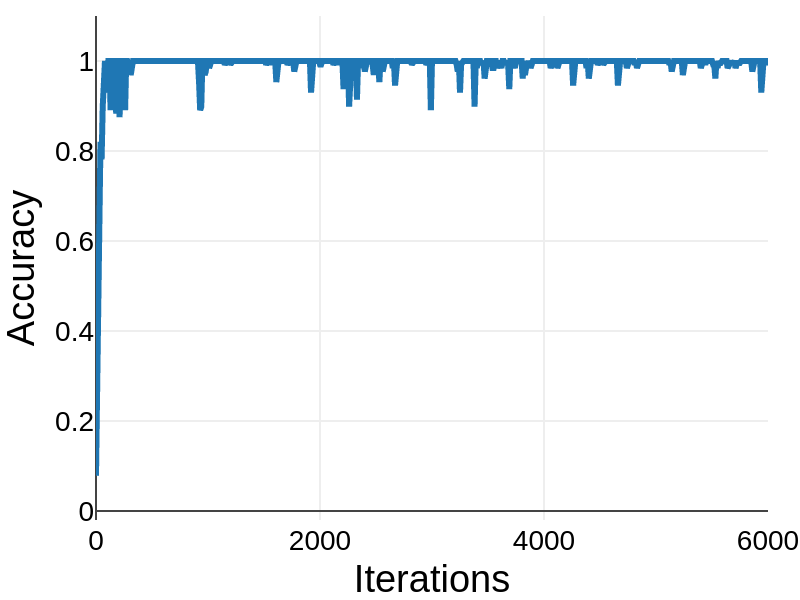
\includegraphics[scale=0.22]{img/rnn-acc-L5}
\caption{}
\end{subfigure}
\begin{subfigure}{0.49\textwidth}
\centering
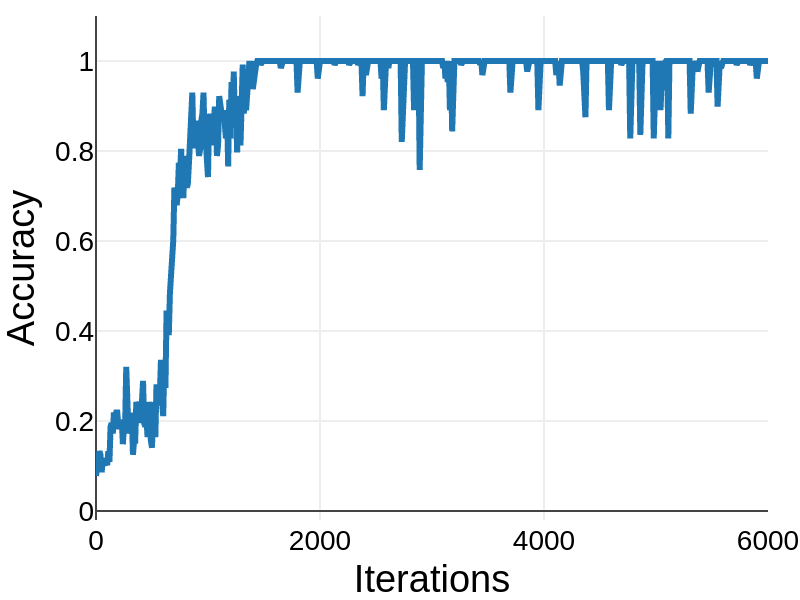
\includegraphics[scale=0.22]{img/rnn-acc-L15}
\caption{}
\end{subfigure}
 \caption{Accuracy curves during training of the RNN, for sequences of (a) length 5, and (b) length 15. While for a length of 5 the model converges quickly to a high accuracy, longer sequences take longer for the model to converge to a good solution.}
\label{fig:rnn_acc_curves}
\end{figure}

\begin{figure}[t]
\centering
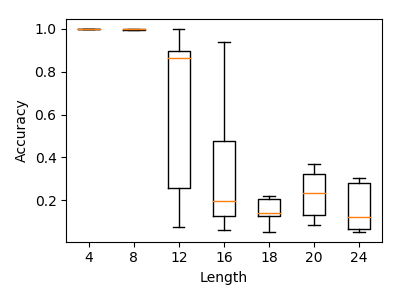
\includegraphics[scale=0.7]{img/rnn-acc-Lbox}
 \caption{Box plots depicting the distribution of the accuracy over 10 runs of the RNN, for different sequence lengths. As the sequence length increases, obtaining a high accuracy is less likely, and longer sequences tend to random performance.}
\label{fig:rnn_acc_box}
\end{figure}

\subsection*{Question 1.4}

When doing optimization with Stochastic Gradient Descent (SGD), we update the parameters in the direction of the gradient of the loss function. This means that two parameter settings for which the gradient is the same, will be updated equally. This can be a limitation if the curvature of the loss function at the two points is different: if the curvature at a point is very low, the update will produce a small change in the loss, while if the curvature is high, the update can make a change too big in the loss function, which might end up at an even higher point. Therefore, it is sensible to include second order information of the gradient that takes into account the curvature of the loss function when updating the parameters.

A direct way to include second order information is to calculate the Hessian matrix, which contains the second derivatives of the loss with respect to all pairs of parameters in the network. As a consequence, evaluating this matrix has a complexity of $O(W^2)$ where $W$ is the number of parameters \cite{bishop2006pattern}. In deep learning, the number of parameters can be on the order of millions, which motivates finding alternative methods that consider curvature in the parameter updates. Two of these include momentum and adaptive learning rate.

When using momentum, we update the parameters with a moving average of the gradient, instead of the gradient only. In this way, every update takes into account previous values of the gradient, producing updates that are smoother than those of SGD.

In SGD, every parameter is updated with the gradient multiplied by the same learning rate. During training, however, some parameters might be near the values of convergence, whereas other still need to be adjusted. It is thus reasonable to adapt the learning rate to each parameter, so that each one is affected only by its own influence on the loss function. Methods like RMSProp implement this by keeping a moving average of the squared gradients, whose inverse is used to multiply the gradient element-wise, effectively adjusting the gradients on different scales for each parameter.

\subsection*{Question 1.5}

In this section we examine the definition of the Long Short-Term Memory (LSTM) network \cite{hochreiter1997lstm} and its implementation.

\begin{description}
\item[a)] The LSTM is comprised by four gates:
\begin{itemize}
\item \textbf{Input modulation gate:} This gate prepares the previous hidden state $\mathbf{h}^{(t-1)}$ and the current input $\mathbf{x}^{(t)}$ to be processed for the current time step. It does so by applying a linear transformation to $\mathbf{h}^{(t-1)}$ and $\mathbf{x}^{(t)}$ and passing the result through a nonlinearity. The nonlinearity is required to give the network the ability to model complex a complex function of its input. The $\tanh$ function is a common choice that limits the range to the interval $(-1, 1)$, and constrains the magnitude of inputs of subsequent layers by saturating for large negative or positive inputs.
\item \textbf{Input gate:} This gate determines the amount of the result of the input modulation gate $\mathbf{g}^{(t)}$ that is used to update the current cell state. This amount is determined by a linear transformation of the previous hidden state $\mathbf{h}^{(t-1)}$ and the current input $\mathbf{x}^{(t)}$, passed through a nonlinearity. In this case a sigmoid is used because it maps its inputs to the interval $(0,1)$, so that $\mathbf{g}^{(t)}$ is not used at all, when the input gate is 0, or used in its entirety, when the input gate is 1. The smooth, monotonic increase of the sigmoid function also allows partial use of $\mathbf{g}^{(t)}$.
\item \textbf{Forget gate:} This gate determines how much of the previous cell state is preserved to update the current cell state, as a function of $\mathbf{h}^{(t-1)}$ and $\mathbf{x}^{(t)}$. A sigmoid is used as the nonlinearity for the same reason as the input gate.
\item \textbf{Output gate:} This gate is used to modulate the amount of the updated current cell state used as the new hidden state $\mathbf{h}^{(t)}$, also as a function of $\mathbf{h}^{(t-1)}$ and $\mathbf{x}^{(t)}$, and using the sigmoid nonlinearity for the same reasons.
\end{itemize}

\item[b)] Let $d$ be the dimension of the input, and $n$ the number of units in the LSTM. There are 8 weight matrices in the LSTM with a size of $(n, d)$, and 4 bias vectors of size $n$. Therefore, the number of trainable parameters in the LSTM cell is $n(8d + 4)$. If we took into account the linear output layer that calculates $\mathbf{p}^{(t)}$, we would have to add $k(h + 1)$ parameterers, where $k$ is the number of outputs.
\end{description}

\subsection*{Question 1.6}

We implemented the LSTM and trained it in the same way as the RNN. Figure \ref{fig:lstm_acc_curves} shows the accuracy curves for sequences of length 5 and 15. We observe that the network reaches an accuracy of 100\% in both cases. Interestingly, for sequences of length 15, the LSTM requires more iterations than the RNN. We attribute this to the increase in the number of parameters.

We also perform experiments for different sequence lengths, as done for the RNN. The results are shown in Figure \ref{fig:lstm_acc_box}, where we observe that the LSTM is much more robust to longer sequences. Only until sequences of length 24 we start observing some variance, but in some runs the model is still able to achieve an accuracy of 100\%. This shows that the LSTM has better memorization capabilities than the RNN, by using its gating mechanisms to control when to retain and forget information from the past.


\begin{figure}[t]
\begin{subfigure}{0.49\textwidth}
\centering
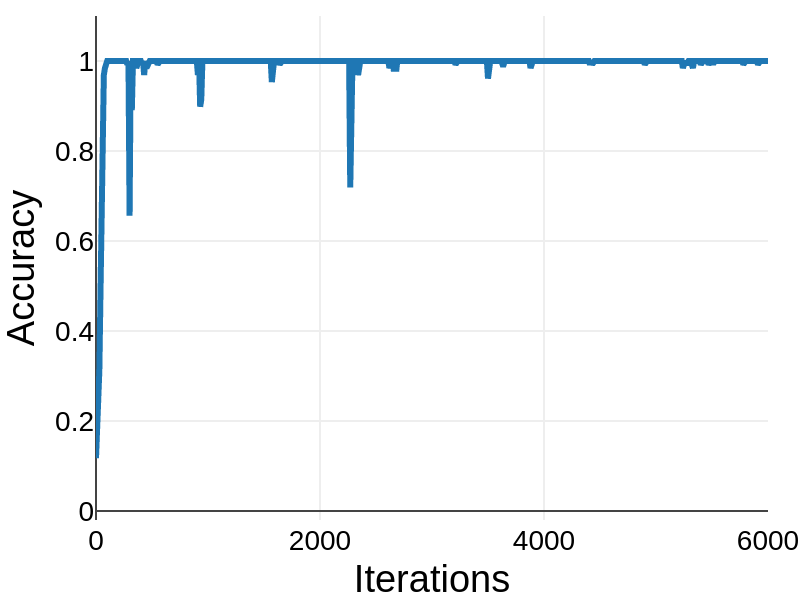
\includegraphics[scale=0.22]{img/lstm-acc-L5}
\caption{}
\end{subfigure}
\begin{subfigure}{0.49\textwidth}
\centering
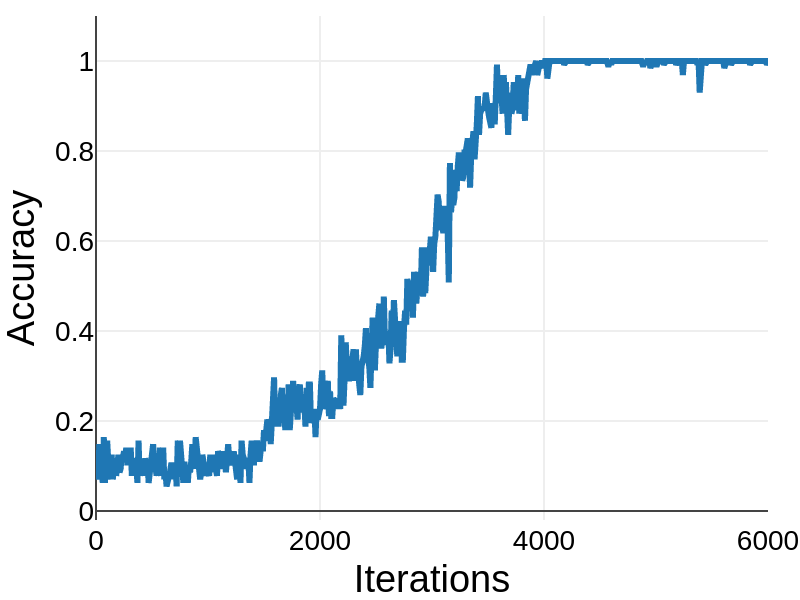
\includegraphics[scale=0.22]{img/lstm-acc-L15}
\caption{}
\end{subfigure}
 \caption{Accuracy curves during training of the LSTM, for sequences of (a) length 5, and (b) length 15. For this setting the LSTM converges more slowly to the solution than the RNN.}
\label{fig:lstm_acc_curves}
\end{figure}

\begin{figure}[t]
\centering
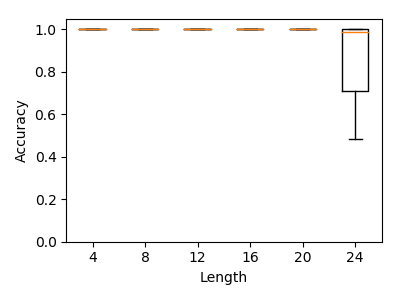
\includegraphics[scale=0.7]{img/lstm-acc-Lbox}
 \caption{Box plots depicting the distribution of the accuracy over 10 runs of the LSTM, for different sequence lengths. The LSTM shows increased robustness to longer sequences compared to the RNN.}
\label{fig:lstm_acc_box}
\end{figure}

\section{Recurrent Nets as Generative Models}

\subsection*{Question 2.1}

\begin{description}
\item[a)] We used PyTorch to train an LSTM network to model text sequences at the character level. In this task, for any character in the sequence, the LSTM needs to predict the next character. The corpus corresponds to the novel \textit{The adventures of Tom Sawyer}, by Mark Twain, which contains 69,693 words.


We use an LSTM with two hidden layers, each with 128 units. The model is trained with the Adam optimizer \cite{kingma2014adam} with a learning rate of 0.002. We use a batch size of 64 sequences, and a maximum sequence length of 30 characters. After training for 100,000 iterations, the model achieves an accuracy of 71.3\%.

\item[b)] During training, we randomly select 5 initial characters to generate samples of sequences of length 30. We do this by feeding the initial character to the LSTM, and then using the character with the maximum probability to feed it to the next step. We show these generated sequences for different steps during training next in Table \ref{tab:lstm-samples}.

At the very beginning of training, we observe that regardless of the initial character, the LSTM generates the same sequences, as it has seen very few examples. In step 1,000 the network already produces some sensible words, but the sequences do not make much sense and they contain mostly the word \texttt{the}, possibly because of its higher frequency compared to other words. The sequence \texttt{sall} appears frequently, a possible explanation is that the sequences \texttt{sa} and \texttt{all the} are very frequent, and the model is starting to learn these short term dependencies, explaining why they end up connected in the sequence \texttt{sall the}.

In step 10,000 we start to observe more interesting sequences. Some of the sentences are grammatical, and they include proper nouns, as shown by the name of the person \texttt{Mary}. Lastly, at iteration 100,000, the meaning behind most of the sequences is clear, and punctuation and contractions are generated as well.


\item[c)] The sequences generated in the previous part are deterministic, as we always choose the next character with the highest probability. We now introduce randomness in the sampling procedure, by drawing characters from a categorical distribution parameterized by the probabilities of the softmax layer. We introduce a \textit{temperature} parameter $T$ that controls the entropy of the distribution: for $T = 0$ the probability of the character with the largest logit is 1, and as we increase $T$,  the distribution will tend to be uniform. The results for multiple values of $T$ are shown in Table \ref{tab:lstm-samples-temp}. We see that at temperatures of 0 and 0.5 the sequences seem to preserve some grammatical structure. As the temperature increases, the sequences make less sense. At a temperature of 2 multiple new line characters appear, as well as symbols like underscores and exclamation marks. We can see clearly that high temperature values introduce more diversity in the sequences, but their meaning is less certain.


\end{description}

\begin{table}[t]
\caption{Samples of text generated by the LSTM at different training steps. The first letter in each sequence is selected uniformly at random.}
\label{tab:lstm-samples}
\centering
\begin{tabular}{p{1.5cm}p{6cm}}
\bf Step & \bf Generated sequences \\
\specialrule{.1em}{.05em}{.05em}
1 & {\texttt{?MMMMMMMMMMMMMMMMMMMMMMMMMMMMM} \nl
\texttt{iMMMMMMMMMMMMMMMMMMMMMMMMMMMMM} \nl
\texttt{bMMMMMMMMMMMMMMMMMMMMMMMMMMMMM} \nl
\texttt{UMMMMMMMMMMMMMMMMMMMMMMMMMMMMM} \nl
\texttt{IMMMMMMMMMMMMMMMMMMMMMMMMMMMMM}} \\
\hline
1,000 & {\texttt{2 the sall the sall the sall t} \nl
\texttt{Ung the sall the sall the sall} \nl
\texttt{Jout the sall the sall the sal} \nl
\texttt{[Tom the sall the sall the sal} \nl
\texttt{No the sall the sall the sall }} \\
\hline
10,000 & {\texttt{But they were a shade of the s} \nl
\texttt{ll they were a shade of the st} \nl
\texttt{Mary in the stranger and the s} \nl
\texttt{xt the same that the words wer} \nl
\texttt{He was a shade of the stranger}} \\
\hline
100,000 & {\texttt{WITHIN a few minutes longer. } \nl
\texttt{nd the stranger of the cave an} \nl
\texttt{I was a little sufferer and th} \nl
\texttt{What'll you take any more of t} \nl
\texttt{ the stranger of the cave and t}} \\
\end{tabular}
\end{table}

\begin{table}[t]
\caption{Samples of generated text for a trained LSTM, with different temperature values. All sequences are initialized with the character \texttt{T}. The new line character is indicated as \texttt{[NL]}.}
\label{tab:lstm-samples-temp}
\centering
\begin{tabular}{p{1cm}p{8cm}}
\bf $T$ & \bf Generated sequences \\
\specialrule{.1em}{.05em}{.05em}
0 & {\texttt{The boys took the first that were the sa}} \\
\hline
0.5 & {\texttt{They showed his little while he was the } \nl
\texttt{The names of the night as he could see t} \nl
\texttt{The boy tools delivered it out of cold h}} \\
\hline
1.0 & {\texttt{Ting-arnic seventemone of coin his tract} \nl 
\texttt{Tom very noon at the other pirates awful} \nl 
\texttt{Tom--they tried hook the night pup, and }} \\
\hline
2.0 & {\texttt{TOy! [NL] \_I'll tap, 'ared But she's on} \nl
\texttt{TOt! [NL] But their Croving emoping Muf} \nl
\texttt{Tom! said Hucko!--whenty-b--swain when[NL]}} \\
\end{tabular}
\end{table}

\subsection*{Question 2.2}

In this section we examine the generation of longer sequences, starting from a specified initial sequence. To do this, we first pass the initial sequence through the LSTM. The final state is used to continue generating characters. Samples of this procedure are shown in Table \ref{tab:lst-long-samples}. We can see that the proper name \texttt{Polly} follows \texttt{Aunt}, and we observed this for different sequences initialized with the same word. This is explained by the fact that in the story, Tom's only aunt is Polly, and she is constantly referred to using this expression.

\begin{table}[t]
\caption{Longer sequences generated by the LSTM given initial sequences (highlighted in bold).}
\label{tab:lst-long-samples}
\centering
\begin{tabular}{p{13cm}}
\hline
\textbf{Aunt} Polly could bear the money was gone, and the stranger of the trees and the stranger of the stranger of the towel in all the time. It seemed to him that if he could not have the stalactite again again. A ghost it must be a pirate. \\
\hline
\textbf{The cave was dark and} the stranger of the stream off and the water to distressed to the stalart with the stranger of the towel in an empty sugar away now.

All right, I reckon they're coming! They're \_tall! You see, said Tom. But there was a sure cautious, maybe--a thousand before they were so grating to the latter temp\\
\hline
\textbf{The water seemed so pleasant that they decided to swim in} the shade of a ha'nted house and benches. No, if it was a sure simpliefs. Tom was to talk at the end of the story of the cave, but the boy could not have the money all the time. I've got it to the wall to him that he was there, and the stranger of the stream off to the wall of the boys.
\end{tabular}
\end{table}

Generally speaking, the sequences are grammatically correct in short contexts, but when considering a broader scope the meaning is lost. This shows that the trained LSTM cannot handle very well complex dependencies over long spans. When given an initial sequence, the generated text that follows is correct but soon the meaning of the initial sequence is lost. This can be seen in all the examples, where the initial sequences mention the word ``aunt'', a cave, and water, but the generated sequences have little connection with them. Lastly, we also observe that some sequences appear with special frequency, as in the case of \texttt{the stranger of}, which suggests that the LSTM might have overfit to this particular sequence.

\section{Graph Neural Networks}

\subsection*{Question 3.1}

\begin{description}
\item[a)] The propagation rule of the GCN is given by the following formula:
\begin{equation}
H^{(l+1)} = \sigma(\hat{A}H^{(l)}W^{(l)})
\label{eq:gcn}
\end{equation}

From this equation, we can see that the network exploits structural information by introducing the adjacency matrix. In a regular, fully connected network, the adjacency matrix is not present in the propagation rule, so each feature in the rows of $H^{(l+1)}$ is only affected by the corresponding row of $H^{(l)}$, dismissing any relationship between a node and its neighbors. By introducing the adjacency matrix in the propagation rule, neighborhood information is taken into account.

To see this, let $h_i^{(l+1)}\in\mathbb{R}^{1\times d}$ be the $i$-th row of $H^{(l+1)}$, corresponding to the feature of node $i$ at layer $l+1$. For simplicity, we have assumed all layers to have the same output dimension $d$. Let $\hat{A}_{i:}$ denote a slice with the $i$-th row of $\hat{A}$. From equation \ref{eq:gcn}, we have:
\begin{align*}
h_i^{(l+1)} &=  \sigma\left(\hat{A}_{i:}H^{(l)}W^{(l)} \right)\\
&= \sigma\left(\sum_{\mathcal{N}(i)} \left(H^{(l)}W^{(l)} \right)_{i:} \right)\\
&= \sigma\left(\sum_{\mathcal{N}(i)} h_i^{(l)}W^{(l)}\right)
\end{align*}

Here $\mathcal{N}(i)$ denotes the set of neighbors of node $i$. Since $\hat{A}$ is a sparse binary matrix, we see that its end effect is to aggregate the features of a node and its neighbors. This can be seen as a form of message passing, where a single forward pass through the GCN layer produces a new feature vector $h_i^{(l+1)}$ for node $i$, that is the result of summing the features of its neighbors and itself, after each one has been multiplied by a weight matrix $W^{(l)}$, and passing the result through a nonlinearity.

\item[b)] As we saw in the previous question, a single layer aggregates features from a node and its immediate neighbors. Therefore, 3 layers are required to propagate information from nodes 3 hops away.
\end{description}

\subsection*{Question 3.2}

Graphs are data structures well suited for applications involving discrete entities and relations between them, to which GNNs can be naturally applied. Examples of these applications include knowledge graphs \cite{nickel2016review,schlichtkrull2018modeling,das2018building}, scene understanding \cite{xu2017scene,herzig2018mapping,liang2018symbolic}, biological interaction networks \cite{hamilton2018embedding}, and citation networks \cite{yang2015network,kipf2016semi,zhang2018diffusion}. Common tasks of interests within these problems include labeling entities according to communities or their structural role, predicting links between entities, and assigning a label to an entity or a graph \cite{hamilton2017representation,bojchevski2017deep,cangea2018towards}. 

GNNs can also be used in chemistry for tasks like drug discovery \cite{gilmer2017nmp}, and in combination with methods like reinforcement learning, they can also be used to generate novel molecules \cite{de2018molgan}.

\subsection*{Question 3.3}

\begin{description}
\item[a)] RNNs are well suited for chain-like sequences, where every element of the sequence is processed after the other, by accumulating the information from the past. This could apply to sequences of words, or frames in a video. In theory, a GNN can also be used in this application as the sequence can be viewed as a chain of nodes, but in order to propagate information from the first element of the sequence to the last, a number of layers equal to the number of elements in the sequence is required, which might not be straightforward in the case of variable-length sequences. Therefore, an RNN would be better suited for this task. 

If a sentence is described in terms of its syntactic tree, a GNN could also be used, but if the tree is large, as before there might not be enough layers in the GNN to propagate information from the leaves to the root of the tree. RNNs, on the other hand, can further be adapted to work with a tree representation of the sentence \cite{tai2015treelstm}, offering a more natural approach to this problem.

When we have a large graph, such as a citation network with publications as nodes, and we want to classify a node in the graph, a DFS or BFS sequential representation is not practical. First, it is based on a prior ordering of the nodes in the tree, and second, for a particular node in the graph, using an RNN to process a DFS or BFS representation would accumulate information from parts of the graph that might not necessary to classify a node, making it harder for the classifier to solve the problem. Instead, an aggregation method that only takes into account a neighborhood of a node is a better solution, which is provided by GNNs.

\item[b)] If we have a scene with multiple entities that are interacting with each other, that changes over time, then a GNN could be used to model the interactions while a recurrent network could aggregate these over time to obtain a relational representation across time. This approach has been used in Relational Recurrent Networks \cite{santoro2017relationalrnn} in tasks such as program evaluation, language modeling and reinforcement learning.

For some problems, the assumption of a static graph does not hold, as multiple nodes and edges can be added or removed through time. A GNN could be extended with a recurrent component to account for changes in the structure of the graph and their effect on future representations. This can be achieved by adding a cell based on the LSTM \cite{manessi2017dynamic,Ma2018StreamingGN}.
\end{description}



\bibliographystyle{unsrt}
\bibliography{refs}
\end{document}
